\documentclass[dvisvgm,border=2mm]{standalone}
\usepackage[T1]{fontenc}
\usepackage{amsmath,amssymb,bm}
\usepackage{mathptmx}
\usepackage{tikz}
\usetikzlibrary{arrows.meta,positioning,fit,backgrounds}

\begin{document}
% DAG 1 — hierarchical structure with partial pooling.
% Same minimal style as the M2 thesis DAG (circle,draw nodes; >=Stealth; ->).
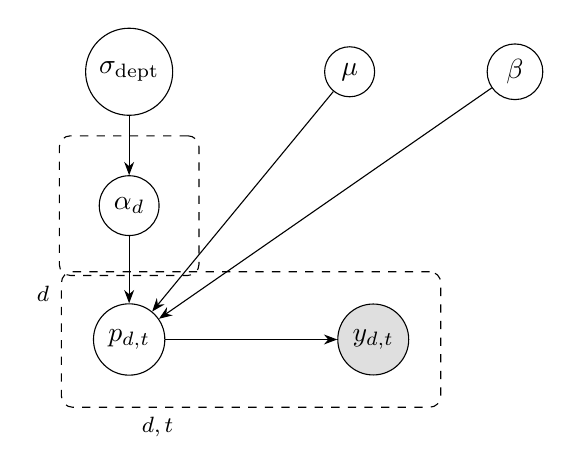
\begin{tikzpicture}[>=Stealth, node distance=1.7cm]
  % hyperparameters (shared across all départements)
  \node[circle, draw] (sig) {$\sigma_{\mathrm{dept}}$};
  \node[circle, draw, right of=sig, xshift=1.1cm] (mu) {$\mu$};
  \node[circle, draw, right of=mu, xshift=0.4cm] (beta) {$\beta$};
  % département effect (one per d)
  \node[circle, draw, below of=sig] (alpha) {$\alpha_d$};
  % cell-level quantities (one per d,t)
  \node[circle, draw, below of=alpha] (p) {$p_{d,t}$};
  \node[circle, draw, fill=gray!25, right of=p, xshift=1.4cm] (y) {$y_{d,t}$};

  \draw[->] (sig)  -- (alpha);
  \draw[->] (alpha) -- (p);
  \draw[->] (mu)   -- (p);
  \draw[->] (beta) -- (p);
  \draw[->] (p)    -- (y);

  \begin{scope}[on background layer]
    \node[draw, rounded corners, dashed, fit=(alpha),
          inner sep=5mm, label={[font=\footnotesize]below left:$d$}] {};
    \node[draw, rounded corners, dashed, fit=(p)(y),
          inner sep=4mm, label={[font=\footnotesize]below left:$d,t$}] {};
  \end{scope}
\end{tikzpicture}
\end{document}
